%% Type de document et encodage de la police
\documentclass[a4paper]{article}
\usepackage[utf8x]{inputenc}
\usepackage[T1]{fontenc}
\usepackage[colorlinks=true, allcolors=black]{hyperref}
% \usepackage[french]{babel}

%% Initialise la taille des pages et des marges
\usepackage[a4paper, top=3cm, bottom=3cm, left=2cm, right=2cm, marginparwidth=2cm]{geometry}

%% Packs utiles
\usepackage{amsmath}
\usepackage{graphicx}

%% Commandes perso
\renewcommand{\arraystretch}{1.2} %% row 20% longer
\renewcommand{\contentsname}{Table des matières}

%% Pour les exemples
\usepackage{mdframed}
\newmdenv[topline=false, bottomline=false, rightline=false, skipabove=\topsep, skipbelow=\topsep]{example}

%% Pour les diagrammes
\usepackage{tikz}
\tikzstyle{incolore} = [rectangle, rounded corners, draw=black, minimum height=1cm, minimum width=3cm, text width=3cm, text centered]


\title{Sécurité des données}
\author{Grégoire Roumache}
\date{Septembre 2020}

\begin{document}

\maketitle

\tableofcontents





\begin{center} \rule{0.90\linewidth}{0.01cm} \end{center}

\textcolor{red}{\textbf{Attention !}} user $ \neq $ login
\begin{itemize}
    \item login = donne accès au serveur (pas aux bases de données)
    \item user = donne accès, à un login, à la base de données
\end{itemize}

\textbf{Remarque}: il n'y a pas de labo 5.















\section{Théorie}










\subsection{Trucs du rappel de base qu'on n'avait pas vu}





\begin{itemize}



\item Une \textbf{vue} est une table virtuelle, elle sert à donner un nom à la requête pour l'utiliser souvent.



\item Une \textbf{procédure stockée} est une instruction SQL précompilée et enregistrée dans la base de données.



\item un \textbf{trigger} est un méchanisme qui permet d'exécuter une fonction/procédure lorsqu'un événement survient.



\item Une \textbf{injection SQL} est une méthode d'exploitation de faille de sécurité. Il s'agit d'injecter du code SQL dans une requête via une entrée de page web.



\item Abréviations:
\begin{itemize}
    \item \textbf{DDL} = Data Definition Language (ex: create, drop)
    \item \textbf{DQl} = Data Query Language (ex: select)
    \item \textbf{DML} = Data Manipulation Language (ex: insert, delete)
    \item \textbf{DCL} = Data Control Language (ex: grant, revoke)
\end{itemize}



\item Créer une vue:
\begin{verbatim}
CREATE VIEW <schema>.<view_name> AS SELECT ...
\end{verbatim}



\item Créer une séquence (peut-être utilisé comme IDENTITY pour créer des valeurs par défaut d'une colonne):
\begin{verbatim}
CREATE SEQUENCE dbo.InvoiceSeq AS INT
    START WITH 1
    INCREMENT BY 1;

-- Récupérer la valeur suivante dans la séquence
SELECT NEXT VALUE FOR dbo.InvoiceSeq;
\end{verbatim}



\end{itemize}










\subsection{Administration}





\begin{itemize}



\item Autorisations:
\begin{itemize}
    \item Accorder une autorisation signifie que l’utilisateur peut accéder à l’objet.
    \item Un refus d’autorisation l’emporte sur un accord d’autorisation. 
\end{itemize}



\item Authentification - Identification:
\begin{itemize}
    \item identification = établir son identité (ex: donner son login)
    \item authentification = prouver son identité (ex: donner son mot de passe)
\end{itemize}



\item Un compte SQL Server est enregistré sur le serveur SQL et n'est pas associé à Active Directory ou Windows.



\item On peut créer un \textbf{compte invité} pour les utilisateurs sans compte enregistré.



\item Chaînage des propriétés (en anglais: \textit{ownership chaining}, pas: \textit{property chaining}):
\begin{itemize}
    \item tous les objets (objets = tables, vues, fonction, etc.) en SQL on un propriétaire
    \item on ne peut accéder à un objet que si on a les autorisations adéquates
    \item quand un objet dépend d'un autre (ex: une vue qui référence une table), une chaîne de propriétés est établie
    \item ça veut dire qu'un utilisateur qui a accès à la vue peut accéder aux données de la table indirectement sans avoir la permission d'accéder à la table directement (seulement si le propriétaire de la table et de la vue est le même utilisateur)
\end{itemize}
\begin{center}
    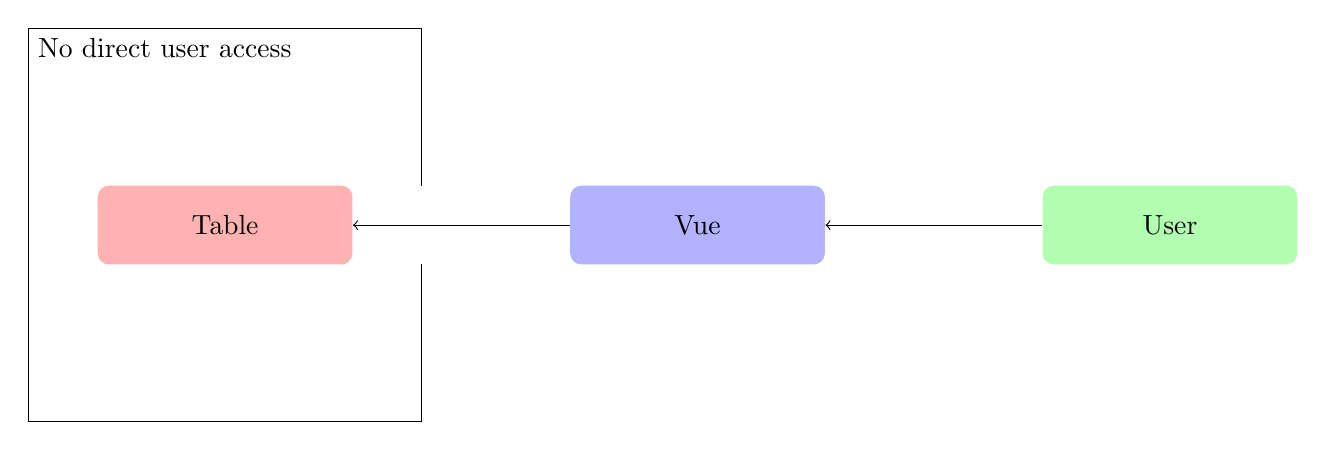
\begin{tikzpicture}

        \node (table) [incolore, draw=none, fill=red!30] at (0,0) {Table};
        \node (vue) [incolore, draw=none, fill=blue!30] at (6,0) {Vue};
        \node (user) [incolore, draw=none, fill=green!30] at (12,0) {User};

        \draw (2.5,0.5) -- (2.5,2.5) -- (-2.5,2.5) -- (-2.5,-2.5) -- (2.5,-2.5) -- (2.5,-0.5);
        \node [anchor=north west] at (-2.5,2.5) {No direct user access};

        \draw[->] (vue) -- (table);
        \draw[->] (user) -- (vue);

    \end{tikzpicture}
\end{center}



\item Types de sauvegardes de base de données:
\begin{itemize}
    \item sauvegarde complète = toutes les données + logs
    \item sauvegarde différentielle = données modifiées/ajoutées sur base de la dernière sauvegarde complète
    \item sauvegarde incrémentielle = données modifiées/ajoutées depuis la dernière sauvegarde (peut être une sauvegarde complète ou incrémentielle)
\end{itemize}



\item L’utilisation de sauvegardes de fichiers accélére la récupération en ne restaurant que les fichiers endommagés sans restaurer le reste de la base de données.



\end{itemize}










\subsection{Protocole SNMP}





\begin{itemize}


\item SNMP = simple network management protocol, sert à:
\begin{itemize}
    \item faire du network monitoring
    \item changer l'état d'un équipement (ex: activer/désactiver une interface)
\end{itemize}


\item 2 types d'entités snmp: les managers et les agents.


\item Manager snmp:
\begin{itemize}
    \item serveur nms (= network management system)
    \item il envoie des requêtes, et reçoit des réponses
    \item il peut aussi recevoir des \textit{traps} (quand quelque chose se passe chez l'agent)
\end{itemize}


\item Agent snmp: service ou démon qui tourne sur une machine.


\item SMI = structure of management information, manière standardisée d'organiser les objets gérés et leur comportement.


\item MIB = management information base, base de donnée des objets gérés par un agent


\item SMI -- MIB:
\begin{itemize}
    \item SMI: ensemble de règles qui définissent la MIB
    \item MIB: Base de donnée des objets
\end{itemize}


\item MIB Remote Monitoring (RMON), collecte des statistiques réseau
\begin{itemize}
    \item La sonde de l'agent collecte les informations et construit les statistiques
    \item Statistiques envoyée à intervalles réguliers ou sur demande du manager
\end{itemize}


\end{itemize}















\section{Pratique}










\subsection{Backup et restauration en 100\% SQL}





\textbf{Remarque}: supprimer la base données avant de la restaurer.

\begin{itemize}



\item Créer un backup en SQL (le dossier \texttt{backup} doit exister):
\begin{verbatim}
USE master
GO
BACKUP DATABASE <nom_db> TO DISK = 'C:\backup\db.bak'
    -- ajouter l'option suivante pour encrypter
    WITH ENCRYPTION (
        ALGORITHM = AES_256,
        SERVER CERTIFICATE = MyCertificate
    )
\end{verbatim}



\item Créer un backup différentiel en SQL:
\begin{verbatim}
-- 1. Créer un backup complet
BACKUP DATABASE <nom_db> TO DISK = 'C:\backup\db_full.bak' WITH INIT;
GO

-- 2. Créer un backup différentiel
BACKUP DATABASE <nom_db> TO 'C:\backup\db_diff.bak' WITH DIFFERENTIAL;
\end{verbatim}



\item Créer une clé d'encryption en SQL (algorithme de chiffrage = AES 256):
\begin{verbatim}
-- Créer la clé de chiffrement (clé principale de chiffrement)
CREATE MASTER KEY ENCRYPTION BY PASSWORD = '23987hxJ#KL95234nl0zBe';
\end{verbatim}



\item Créer un certificat en SQL (attention changer la date d'expiration):
\begin{verbatim}
-- Ouvrir la clé principale de chiffrement dans la session où on crée le certificat
OPEN MASTER KEY DECRYPTION BY PASSWORD = '23987hxJ#KL95234nl0zBe'

-- Créer le certificat encrypté avec la clé de chiffrement principale
CREATE CERTIFICATE MyCertificate
    WITH SUBJECT = 'Backup certificate',
    EXPIRY_DATE = '20201031';
\end{verbatim}



\item Restaurer une base de données en SQL:
\begin{verbatim}
USE master
GO
RESTORE DATABASE <nom_db> FROM DISK = 'C:\backup\db.bak'
\end{verbatim}



\item Restaurer une base de données différentielle en SQL:
\begin{verbatim}
-- 1. Restaurer la base de données complète (avec l'option NORECOVERY)
RESTORE DATABASE <nom_db> FROM DISK = 'C:\backup\db_full.bak'
   WITH NORECOVERY;
GO

-- 2. Restaurer le backup différentiel
RESTORE DATABASE <nom_db> FROM DISK = 'C:\backup\db_diff.bak'
   WITH FILE = 2,
   RECOVERY;
\end{verbatim}



\end{itemize}










\subsection{Backup et restauration en 100\% UI}





\textbf{Remarque}: supprimer la base données avant de la restaurer.

\begin{itemize}



\item Créer un backup dans l'UI:
\begin{enumerate}
    \item click-droit sur la base de données, click sur \textit{tasks}, click sur \textit{back-up}
    \item choisir le type avec l'option \textit{backup style} (\textit{full} ou \textit{differential})
    \item en bas à droite, click sur \textit{add} pour sélectionner l'emplacement du backup
    \item pour écraser le backup précédent, sélectionner \textit{media options} dans le menu de gauche et click sur \textit{back up to a new media set and erase all existing backup sets}
    \item pour encrypter le backup, sélectionner \textit{backup options} dans le menu de gauche, click sur \textit{encrypt backup}, sélectionner l'algorithme et le certificat
\end{enumerate}
\textbf{Remarque}: pour encrypter le backup, il faut écraser les backups précédents.



\item Restaurer une base de données dans l'UI:
\begin{enumerate}
    \item dans le menu de gauche, click-droit sur \textit{databases}, puis click sur \textit{restore database}
    \item sélectionner l'option \textit{device}, puis click sur \textit{...} à droite
    \item ensuite, click sur \textit{Add} et sélectionner le fichier de backup
    \item si vous restaurez àpd backup différentiel, ajouter le fichier de backup complet et le fichier différentiel
\end{enumerate}



\item Générer un script de restauration:
\begin{enumerate}
    \item click-droit sur la base de données, puis click sur \textit{tasks}, puis sur \textit{generate scripts}
    \item pour ne restaurer que les tables, dans le menu \textit{choose objects}, sélectionner l'option \textit{select specific database objects} et sélectionner \textit{tables}
\end{enumerate}
\textbf{Remarques}:
\begin{itemize}
    \item supprimer la base de données avant de la restaurer avec le script
    \item pour ne restaurer que les tables, supprimer uniquement les tables
\end{itemize}



\end{itemize}










\subsection{Authentifications et autorisations}





\begin{itemize}


\item Créer un login:
\begin{itemize}
    \item Compte windows: \texttt{CREATE LOGIN [<domain>/<login>] FROM WINDOWS}
    \item Compte SQL: \texttt{CREATE LOGIN <login> WITH PASSWORD = '<password>'}
\end{itemize}


\item Afficher la liste des rôles:
\begin{itemize}
    \item Tous les rôles: \texttt{EXEC sp\_helprole}.
    \item Rôles par défaut de la DB: \texttt{EXEC sp\_helpsrvrole}.
\end{itemize}


\end{itemize}










\subsection{Automatisation, Audit, Optimisation}





\begin{itemize}



\item Pour avoir des jobs automatisés, il faut activer le SQL Server Agent:
\begin{enumerate}
    \item dans le menu de gauche, faire un clic droit sur \textit{SQL Server Agent}
    \item cliquer sur \textit{start}, ensuite cliquer sur \textit{yes} dans toutes les fenêtres pop up
\end{enumerate}



\item Créer un job:
\begin{enumerate}
    \item dans le menu de gauche, faire un clic droit sur \textit{SQL Server Agent/Jobs}
    \item cliquer sur \textit{new job}
    \item dans \textit{general}, donner un nom au job
    \item dans \textit{steps}:
    \begin{enumerate}
        \item cliquer sur \textit{new}
        \item donner un nom à la step
        \item dans \textit{command}, mettre la query SQL à exécuter
        \item appuyer sur \textit{ok}
    \end{enumerate}
    \item dans \textit{schedules}:
    \begin{enumerate}
        \item cliquer sur \textit{new}
        \item donner un nom au schedule
        \item configurer le moment d'exécution
        \item appuyer sur \textit{ok}
    \end{enumerate}
    \item appuyer sur \textit{ok}
\end{enumerate}



\item Ouvrir SQL Profiler : dans le menu du haut, cliquer sur \textit{tools}, puis \textit{SQL Profiler}.



\item Analyser des requêtes:
\begin{enumerate}
    \item sélectionner la requête, puis faire un clic droit
    \item cliquer sur \textit{display estimated execution plan}
\end{enumerate}



\end{itemize}










\subsection{Vérifications SQL}





\begin{itemize}



\item Afficher les logins:
\begin{verbatim}
SELECT name, type, type_desc FROM master.sys.sql_logins
\end{verbatim}



\item Afficher les utilisateurs:
\begin{verbatim}
SELECT * FROM sysusers
\end{verbatim}



\item Afficher les rôles:
\begin{verbatim}
SELECT name FROM sys.database_principals WHERE type = 'R'
\end{verbatim}



\item Afficher les rôles et leurs membres:
\begin{verbatim}
SELECT DP1.name AS RoleName, isnull (DP2.name, '/') AS UserName
FROM sys.database_role_members AS DRM
RIGHT OUTER JOIN sys.database_principals AS DP1 ON DRM.role_principal_id = DP1.principal_id
LEFT OUTER JOIN sys.database_principals AS DP2 ON DRM.member_principal_id = DP2.principal_id
ORDER BY DP1.name
\end{verbatim}



\item Afficher les bases de données:
\begin{verbatim}
SELECT name FROM master.dbo.sysdatabases
\end{verbatim}



\item Afficher les permissions d'un utilisateur:
\begin{verbatim}
SELECT * FROM fn_my_permissions('<user>', 'USER')
\end{verbatim}



\end{itemize}




















\appendix \newpage




















\section{Labo 3 -- Authentification \& Autorisation des Utilisateurs}





\begin{itemize}



\item Exercice 1 -- Créer différents 'logins' SQL qui utiliseront plusieurs méthodes d’authentification:
\begin{itemize}

\item Utiliser CMD pour localiser l'utilisateur et ses groupes locaux de sécurité.
\begin{example}
Dans CMD: \texttt{whomai /groups}
\end{example}

\item Utiliser T-SQL pour créer un login d’authentification de type 'SQL Server' nommé 'UsrSQL'.
\begin{example} \begin{verbatim}
CREATE LOGIN UsrSQL WITH PASSWORD = '<password>';
\end{verbatim} \end{example}

\item Utiliser SMS pour créer un login de type 'Windows Authenticated' de l'AD (etuXXXXX).
\begin{example} \begin{verbatim}
CREATE LOGIN [<domain>\<login>] FROM WINDOWS;
\end{verbatim} \end{example}

\item Utiliser T-SQL pour ajouter votre login AD dans le rôle fixe du server 'setupadmin'.
\begin{example}
    \textcolor{red}{\textbf{Attention !}} Erreur du prof car, on ne peut ajouter que des utilisateurs à un rôle, pas des logins.    
\end{example}
\begin{example} \begin{verbatim}
-- EXEC sp_addrolemember @rolename = setupadmin, @membername = UserSQL;
    -- => "do not have permission"
-- ALTER ROLE setupadmin ADD MEMBER UserSQL;
    -- => "do not have permission"
==> clic-droit sur <server>/security/logins/UsrSQL
==> properties -> server roles -> setupadmin -> ok
\end{verbatim} \end{example}

\item Utiliser SSMS pour ajouter le login ‘UsrSQL’ dans le rôle fixe du server 'bulkadmin'.
\begin{example} \begin{verbatim}
==> clic-droit sur <server>/security/logins/UsrSQL
==> properties -> server roles -> bulkadmin -> ok
\end{verbatim} \end{example}

\item Utiliser la bonne procédure stockée qui vérifie l'appartenance au niveau des groupes.
\begin{example} \begin{verbatim}
EXEC sp_helprolemember <role>;
EXEC sp_helpsrvrolemember <role>; -- rôles serveur
\end{verbatim} \end{example}

\end{itemize}



\item Exercice 2 -- Créer différents 'rôles' définis au niveau du server SQL:
\begin{itemize}

\item Utiliser SMS pour créer un rôle défini nommé 'LoginManager'.
\begin{example} \begin{verbatim}
==>  clic-droit sur <server>/databases/<database>/security/roles/database roles
==> -> new database role -> role name -> ok
\end{verbatim} \end{example}

\item Permettre à ce rôle d'accorder la permission 'ALTER ANY LOGIN'.
\begin{example} \begin{verbatim}
GRANT ALTER ANY LOGIN TO UserSQL;
\end{verbatim} \end{example}

\item Ajouter votre utilisateur AD ou local dans ce rôle défini.
\begin{example} \begin{verbatim}
ALTER ROLE LoginManager ADD MEMBER UserSQL;
\end{verbatim} \end{example}

\item Utiliser T-SQL pour créer un rôle défini nommé 'CreatorManager'.
\begin{example} \begin{verbatim}
EXEC sp_addrole @rolename = 'CreatorManager';
-- CREATE ROLE CreatorManager;
\end{verbatim} \end{example}

\item Permettre à ce rôle d’accorder la permission 'CREATE ANY DATABASE'.
\begin{example} \begin{verbatim}
USE master;
GO
GRANT CREATE ANY DATABASE TO CreatorManager;
\end{verbatim} \end{example}

\item ajouter l’utilisateur ‘UsrSQL’ dans ce rôle avec T-SQL.
\begin{example} \begin{verbatim}
EXEC sp_addrolemember @rolename = 'CreatorManager', @membername = 'UserSQL';
-- ALTER ROLE CreatorManager ADD MEMBER UserSQL;
\end{verbatim} \end{example}

\end{itemize}



\item Exercice 3 -- Créer différents ‘utilisateurs’ définis au niveau des bases de données basés sur les ‘logins’ créés précédemment:
\begin{itemize}

\item Utiliser SSMS pour ajouter votre login AD dans le rôle 'db\_datareader' pour la DB 'AdventureWorks'.
\begin{example} \begin{verbatim}
==> clic-droit sur <serveur>/security/logins/<login> -> properties
==> -> user mapping -> AdventureWorks -> db_datareader -> ok
\end{verbatim} \end{example}

\item Utiliser T-SQL pour créer un role au niveau de la DB nommé ‘TableAdmin’ pour la DB ‘AdventureWorks’.
\begin{example} \begin{verbatim}
USE AdventureWorks;
GO
EXEC sp_addrole @rolename = 'TableAdmin';
-- CREATE ROLE TableAdmin;
\end{verbatim} \end{example}

\item Donner les permissions 'CREATE TABLE' et 'CREATE SCHEMA' au rôle 'TableAdmin'
\begin{example} \begin{verbatim}
GRANT CREATE TABLE, CREATE SCHEMA TO TableAdmin;
\end{verbatim} \end{example}

\end{itemize}



\item Exercice 4 -- Configurer les permissions au niveau des bases de données, schémas et rôles.
\begin{itemize}

\item S’identifier sur l’instance par défaut avec l’utilisateur 'KimPossible'.
\begin{example}
\begin{enumerate}
    \item Créer l'utilisateur \textit{KimPossible}: \\
    \texttt{CREATE LOGIN KimPossible WITH PASSWORD = '<password>';}
    \item Se connecter avec \textit{KimPossible}: \\
    \texttt{SETUSER KimPossible;} \\
    Si ça ne marche pas, il faut se connecter avec SSMS \\
    \texttt{==> clic-droit sur <serveur> -> connect}.
\end{enumerate}
\end{example}

\item Créer une nouvelle base de données nommée ‘Middleton’.
\begin{example} \begin{verbatim}
CREATE DATABASE MiddleTon;
\end{verbatim} \end{example}

\item Créer un nouveau rôle nommé ‘TeamImpossible’.
\begin{example} \begin{verbatim}
CREATE ROLE TeamImpossible;
\end{verbatim} \end{example}

\item Créer 3 tables nommés par défaut ‘Website’, ‘Babysitting’, ‘LowMowning’.
\begin{example} \begin{verbatim}
CREATE TABLE Website (Id INT);
CREATE TABLE Babysitting (Id INT);
CREATE TABLE LowMowning (Id INT);
\end{verbatim} \end{example}

\item Créer un nouveau schéma nommé ‘KimServices’.
\begin{example} \begin{verbatim}
CREATE SCHEMA KimServices;
\end{verbatim} \end{example}

\item Octroyer au rôle ‘TeamImpossible’ les privilèges suivants ‘SELECT’ ‘REFERENCES’ ‘INSERT’ ‘UPDATE’ ‘DELETE’ et ‘VIEW DEFINITION’ sur le schéma ‘KimServices’ 
\begin{example} \begin{verbatim}
GRANT SELECT, REFERENCES, INSERT, UPDATE, DELETE, VIEW DEFINITION
TO KimServices;
\end{verbatim} \end{example}

\end{itemize}



\item Commandes pour annuler tout ce qui a été modifié dans ce labo:
\begin{example} \begin{verbatim}
    -- Exercice 1
DROP LOGIN UserSQL;
DROP LOGIN [<domain>\<login>];
    -- Exercice 2
DROP ROLE LoginManager;
DROP ROLE CreatorManager;
    -- Exercice 3
USE AdventureWorks;
GO
DROP ROLE TableAdmin;
    -- Exercice 4
DROP DATABASE Middleton;
\end{verbatim} \end{example}



\end{itemize}















\section{Labo 4 -- Gestion des Accès}





\begin{itemize}



\item À partir d’un besoin client :
\begin{itemize}
    \item Établir la liste des utilisateurs devant avoir accès aux bases de données.
    \item Regrouper des objets de bases de données en schéma.
    \item Définir les permissions des utilisateurs pour chaque objet de bases de données.
    \item Établir une matrice des rôles qui fait le lien entre les utilisateurs et les objets de bases de données.
\end{itemize}



\item Exercice:
\begin{enumerate}


\item Lister les utilisateurs et les comptes pour chaque base de données.
\begin{example}
    Utilisateurs:
    \begin{itemize}
        \item Patrick, président
        \item André, administrateur système
        \item Pierre, responsable du refuge des champs
        \item Paul, responsable du refuge des prés
        \item Jacques, responsable du refuge des plages
        \item Jean, responsable du refuge des plaines
        \item 1 responsable des inscriptions, dans chaque refuge
        \item 1 médecin, dans l'association
        \item 1 soigneur, dans l'association
        \item les utilisateurs externes
    \end{itemize}
\end{example}


\item Attribuer les rôles serveur et de base de données pour chaque utilisateur.
\begin{example}
    Rôles:
    \begin{itemize}
        \item président
        \item administrateur système
        \item responsable du refuge
        \item responsable des inscriptions
        \item médecin
        \item soigneur
        \item utilisateurs externes
    \end{itemize}
\end{example}


\item Créer la matrice des rôles (pour chaque base de données) en respectant le canevas.
\begin{example}
    Matrice des \textbf{autorisations}:
    \begin{center}
        \begin{tabular}{|c|c|c|c|c|} \hline
            & select & insert & update & delete \\ \hline
            président & * & * & * & * \\
            administrateur système & * & * & * & * \\
            responsable du refuge & * & * & * & * \\
            responsable des inscriptions & A,R & A & A & / \\
            médecin & A,R,S & S & A,S & S \\
            soigneur & A,R,S & S & S & / \\
            utilisateurs externes & A,R & / & / & / \\ \hline
        \end{tabular}
    \end{center}
    * = tout, A = animal, L = localisation, S = soin
\end{example}


\item Créer les 4 bases de données ainsi que les utilisateurs en respectant la matrice des rôles.
\begin{example}

\begin{itemize} \item Restaurer la base de données 4 fois: \end{itemize}
\begin{verbatim}
USE master
GO
RESTORE DATABASE HENACCUEIL1 FROM DISK = 'C:\backup\db.bak'

-- Remarque: Si on essaie de restaurer une 2ème fois la même base de données,
-- ça va donner des erreurs et pointer vers les fichiers logiques à modifier,
-- ici: 'Examen', 'Examen_log'

RESTORE DATABASE HENACCUEIL2 FROM DISK = 'E:\HENACCUEIL.bak' WITH
    MOVE 'Examen' TO 'E:\HENACCUEIL2',
    MOVE 'Examen_log' TO 'E:\HENACCUEIL2_log'
GO

RESTORE DATABASE HENACCUEIL3 FROM DISK = 'E:\HENACCUEIL.bak' WITH
    MOVE 'Examen' TO 'E:\HENACCUEIL3',
    MOVE 'Examen_log' TO 'E:\HENACCUEIL3_log'
GO

RESTORE DATABASE HENACCUEIL4 FROM DISK = 'E:\HENACCUEIL.bak' WITH
    MOVE 'Examen' TO 'E:\HENACCUEIL4',
    MOVE 'Examen_log' TO 'E:\HENACCUEIL4_log'
GO
\end{verbatim}

\begin{itemize} \item Créer les logins: \end{itemize}
\begin{verbatim}
CREATE LOGIN Patrick WITH PASSWORD = 'password'
CREATE LOGIN Andre   WITH PASSWORD = 'password'
CREATE LOGIN Pierre  WITH PASSWORD = 'password'
CREATE LOGIN Paul    WITH PASSWORD = 'password'
CREATE LOGIN Jacques WITH PASSWORD = 'password'
CREATE LOGIN Jean    WITH PASSWORD = 'password'
\end{verbatim}

\begin{itemize} \item Créer les utilisateurs: \end{itemize}
\begin{verbatim}
CREATE USER Patrick
CREATE USER <responsable_du_refuge>
CREATE USER Jean
\end{verbatim}

\begin{itemize} \item Créer les rôles: \end{itemize}
\begin{verbatim}
CREATE ROLE President
CREATE ROLE AdministrateurSysteme
CREATE ROLE ResponsableRefuge
CREATE ROLE ResponsableInscriptions
CREATE ROLE Medecin
CREATE ROLE Soigneur
-- utilisateurs externes = pas de rôle
\end{verbatim}

\begin{itemize} \item Ajouter les utilisateurs aux rôles: \end{itemize}
\begin{verbatim}
ALTER ROLE President             ADD MEMBER Patrick
ALTER ROLE AdministrateurSysteme ADD MEMBER André
ALTER ROLE ResponsableRefuge     ADD MEMBER <responsable_du_refuge>
\end{verbatim}

\begin{itemize} \item Donner les permissions aux rôles: \end{itemize}
\begin{verbatim}
-- par défaut: DENY ALL ON ALL TO PUBLIC
GRANT ALL ON ALL TO President, AdministrateurSysteme, ResponsableRefuge

GRANT SELECT, INSERT, UPDATE ON ANIMAL TO ResponsableInscriptions
GRANT SELECT ON REFUGE TO ResponsableInscriptions

GRANT SELECT, UPDATE ON ANIMAL TO Medecin
GRANT SELECT ON REFUGE TO Medecin
GRANT ALL ON SOIN TO Medecin

GRANT SELECT ON ANIMAL, REFUGE TO Soigneur
GRANT SELECT, INSERT, UPDATE ON SOIN TO Soigneur

GRANT SELECT ON ANIMAL, REFUGE TO PUBLIC
\end{verbatim}

\end{example}

\end{enumerate}



\item Commandes pour annuler tout ce qui a été modifié dans ce labo:
\begin{example} \begin{verbatim}
DROP LOGIN Patrick
DROP LOGIN Andre
DROP LOGIN Pierre
DROP LOGIN Paul
DROP LOGIN Jacques
DROP LOGIN Jean
-- montrer tous les logins
SELECT name, type, type_desc FROM master.sys.sql_logins

DROP ROLE President
DROP ROLE AdministrateurSysteme
DROP ROLE ResponsableRefuge
DROP ROLE ResponsableInscriptions
DROP ROLE Medecin
DROP ROLE Soigneur
-- montrer tous les rôles et les utilisateurs membres
SELECT DP1.name AS RoleName, isnull (DP2.name, '/') AS UserName
    FROM sys.database_role_members AS DRM
    RIGHT OUTER JOIN sys.database_principals AS DP1
        ON DRM.role_principal_id = DP1.principal_id
    LEFT OUTER JOIN sys.database_principals AS DP2
        ON DRM.member_principal_id = DP2.principal_id
    ORDER BY DP1.name
-- montrer tous les rôles
SELECT name FROM sys.database_principals WHERE type = 'R' -- R = rôle

DROP DATABASE HENACCUEIL1
DROP DATABASE HENACCUEIL2
DROP DATABASE HENACCUEIL3
DROP DATABASE HENACCUEIL4
-- montrer toutes les bases de données
SELECT * FROM master.dbo.sysdatabases
\end{verbatim} \end{example}



\end{itemize}















\section{Labo 6 -- Index}





\begin{itemize}



\item Restaurer la base de données.
\begin{example} \begin{verbatim}
USE master
GO
RESTORE DATABASE BigDB FROM DISK = 'E:\databases\bigDB_Light.bak'
\end{verbatim} \end{example}



\item Supprimer le cache de SQL Server.
\begin{example} \begin{verbatim}
CHECKPOINT
GO
DBCC DROPCLEANBUFFERS
\end{verbatim} \end{example}



\item Activer la mesure du temps d'exécution des requêtes.
\begin{example} \begin{verbatim}
SET STATISTICS TIME ON
\end{verbatim} \end{example}



\item Exercice 1:
\begin{itemize}
\item Exécuter la requête suivante : \texttt{SELECT COUNT(*) FROM users WHERE age < 50} (4956 ms)
\item Créer un index pour accélérer la requête et mesurer le temps d'exécution.
\begin{example} \begin{verbatim}
-- essayer avec l'age
-- essayer avec l'id
-- essayer avec l'id + age
-- essayer avec l'id + la condition
-- essayer avec l'age + la condition
CREATE INDEX i1 ON users(age)                -- build = 247116 ms, select =  389 ms
CREATE INDEX i2 ON users(id)                 -- build =  75506 ms, select = 4821 ms
CREATE INDEX i3 ON users(id, age)            -- build =  99161 ms, select = 1566 ms
CREATE INDEX i4 ON users(id) WHERE age < 50  -- build =  59025 ms, select =  459 ms
CREATE INDEX i5 ON users(age) WHERE age < 50 -- build = 137070 ms, select =  387 ms
                                             -- sans index,        select = 4956 ms
                                             -- sans index, cache, select = 1641 ms
\end{verbatim} \end{example}
\end{itemize}



\item Exercice 2:
\begin{itemize}
\item Exécuter la requête suivante : \texttt{SELECT * FROM users WHERE age > 99}
\item Désactiver l'index de l'exercice 1.
\begin{example} \begin{verbatim}
ALTER INDEX i1 ON users DISABLE
\end{verbatim} \end{example}
\item Créez un index plus petit que celui de l'exercice 1 et qui donnera les mêmes performances.
\begin{example} \begin{verbatim}
CREATE INDEX i6 ON users(age) WHERE age > 99
SELECT * FROM users WHERE age > 99      -- build = 1977 ms, select =   58 ms
                                        -- sans index,      select = 4944 ms
\end{verbatim} \end{example}
\item Utiliser l'instruction suivante pour voir la taille des index de la db:
\begin{verbatim}
SELECT
    i.[name] AS IndexName,
    SUM(s.[used_page_count]) * 8 AS IndexSizeKB
FROM
    sys.dm_db_partition_stats AS s
INNER JOIN
    sys.indexes AS i
ON
    s.[object_id] = i.[object_id]
    AND s.[index_id] = i.[index_id]
GROUP BY i.[name]
ORDER BY i.[name]
GO
\end{verbatim}
\item Comparer la taille des index des exercices 1 et 2.
\begin{example} \begin{verbatim}
- i1 = 1'387'672 ko
- i2 =   990'616 ko
- i3 = 1'387'680 ko
- i4 =   490'432 ko
- i5 =   686'952 ko
- i6 =     6'968 ko
\end{verbatim} \end{example}
\end{itemize}



\item Exercice 3:
\begin{itemize}
\item Exécutez la requête suivante : \texttt{SELECT TOP 100 * FROM users ORDER BY nom DESC, prenom DESC, age ASC}
\item Créez des index sur nom, prénom et sur âge. Exécutez, ensuite, à nouveau la requête.
\begin{example} \begin{verbatim}
CREATE INDEX i7 ON users(nom)
CREATE INDEX i8 ON users(prenom)
CREATE INDEX i1 ON users(age)       -- existe déjà
\end{verbatim} \end{example}
\item Créez un seul nouvel index qui sera vraiment efficace (penser à un annuaire).
\begin{example} \begin{verbatim}
CREATE INDEX i9 ON users(nom DESC, prenom DESC, age ASC)
\end{verbatim} \end{example}
\end{itemize}



\item Exercice 4:
\begin{itemize}
\item Regarder la place que les index prennent sur le disque dur.
\begin{enumerate}
    \item Clic droit sur la base de données.
    \item Cliquer sur \textit{Reports}.
    \item Cliquer sur \textit{Standard Reports}.
    \item Cliquer sur \textit{Disk Usage by Top Tables}.
\end{enumerate}
\item Comparez l’espace occupé par les index avec l’espace pris par la table.
\begin{example} \begin{verbatim}
- user = 6'199'284 ko
-   i1 = 1'387'672 ko (index le plus large)
\end{verbatim} \end{example}
\end{itemize}



\item Commandes pour annuler tout ce qui a été modifié dans ce labo:
\begin{example} \begin{verbatim}
DROP INDEX i1 ON users
DROP INDEX i2 ON users
DROP INDEX i3 ON users
DROP INDEX i4 ON users
DROP INDEX i5 ON users
DROP INDEX i6 ON users
DROP INDEX i7 ON users
DROP INDEX i8 ON users
DROP INDEX i9 ON users
SET STATISTICS TIME OFF
USE master
DROP DATABASE BigDB
\end{verbatim} \end{example}



\end{itemize}















\section{Labo 7 -- Audit et journalisation}





\begin{itemize}



\item Restaurez la base de données présente sur Moodle.
\begin{example} \begin{verbatim}
USE master
RESTORE DATABASE SecuData FROM DISK = 'E:\databases\DB_SecuData_Audit.bak'
\end{verbatim} \end{example}



\item Créer les utilisateurs:
\begin{itemize}
    \item Créez un utilisateur avec un mot de passe respectant la stratégie évoquée plutôt, en lui donnant le rôle le plus approprié et l’accès en lecture sur la table Personne.
    \item Créez un autre utilisateur qui aura les droits propriétaires sur la base de données.
\end{itemize}
\begin{example} \begin{verbatim}
USE SecuData
CREATE LOGIN User1 WITH PASSWORD = '??Password007??'
CREATE LOGIN User2 WITH PASSWORD = '??Password007??'
GO
CREATE USER User1
CREATE USER User2
GO
GRANT SELECT ON Personne TO User1
GRANT ALL ON DATABASE::SecuData TO User2
GO
\end{verbatim}
\textbf{Remarque}:
\begin{itemize}
    \item le prof avait déjà créé les utilisateurs \textit{user1}, et \textit{user2}
    \item il faut les supprimer puis les rajouter
\end{itemize}
\end{example}






\item Créez un Audit pour chacun des utilisateurs.
\begin{itemize}
    \item Pour le premier : le type d’action ciblera les Select et les Insert.
    \item Pour le second : le type d’action ciblera les Execute et les Delete.
\end{itemize}
\begin{example}
    \begin{verbatim}
USE master
CREATE SERVER AUDIT AuditManip1
TO FILE (FILEPATH = 'E:\databases\')
ALTER SERVER AUDIT AuditManip1 WITH (STATE = ON);
CREATE SERVER AUDIT AuditManip2
TO FILE (FILEPATH = 'E:\databases\')
ALTER SERVER AUDIT AuditManip2 WITH (STATE = ON);
        
USE SecuData
CREATE DATABASE AUDIT SPECIFICATION AuditManip1Specification
FOR SERVER AUDIT AuditManip1
ADD (SELECT ON DATABASE::SecuData BY User1),
ADD (INSERT ON DATABASE::SecuData BY User1)
WITH (STATE = ON);
CREATE DATABASE AUDIT SPECIFICATION AuditManip2Specification
FOR SERVER AUDIT AuditManip2
ADD (EXECUTE ON DATABASE::SecuData BY User2),
ADD (DELETE  ON DATABASE::SecuData BY User2)
WITH (STATE = ON);
    \end{verbatim}
\end{example}



\item Affichez les noms et les prénoms des personnages ayant 16 ans avec le premier utilisateur.
\begin{example} \begin{verbatim}
EXECUTE AS USER = 'User1'
SELECT nom, prenom FROM personnages WHERE age = 16
REVERT
\end{verbatim} \end{example}



\item Ajoutez une ligne dans la table Personne avec le second utilisateur et supprimez la ligne avec l’ID = 1.
\begin{example} \begin{verbatim}
EXECUTE AS USER = 'User2'
INSERT INTO Personne (nom, prenom, age) VALUES ('Grégoire', 'Roumache', 21)
DELETE FROM Personne WHERE id = 1
REVERT
\end{verbatim} \end{example}



\item Consultez les journaux d’audit.
\begin{example}
    \begin{enumerate}
        \item Dans SSMS, faire un clic droit sur \textit{<serveur>/security/audits/<audit>}.
        \item Cliquer sur \textit{view audit logs} (\textit{afficher les journaux d'audit}).
    \end{enumerate}
\end{example}



\item Commandes pour annuler tout ce qui a été modifié dans ce labo:
\begin{example} \begin{verbatim}
USE SecuData
ALTER DATABASE AUDIT SPECIFICATION AuditManip1Specification WITH (STATE = OFF)
ALTER DATABASE AUDIT SPECIFICATION AuditManip2Specification WITH (STATE = OFF)
DROP DATABASE AUDIT SPECIFICATION AuditManip1Specification
DROP DATABASE AUDIT SPECIFICATION AuditManip2Specification
USE master
ALTER SERVER AUDIT AuditManip1 WITH (STATE = OFF);
ALTER SERVER AUDIT AuditManip2 WITH (STATE = OFF);
DROP SERVER AUDIT AuditManip1
DROP SERVER AUDIT AuditManip2
DROP LOGIN User1
DROP LOGIN User2
GO
DROP DATABASE SecuData
\end{verbatim} \end{example}



\end{itemize}















\section{Labo 8}





Si vous avez ce problème sous Debian : "Bad operator (INTEGER): At line 73 in /usr/share/snmp/mibs/ietf/SNMPv2-PDU"

Voici la commande qui peut réparer l'erreur : "wget http://pastebin.com/raw.php?i=p3QyuXzZ \\-O /usr/share/snmp/mibs/ietf/SNMPv2-PDU"




















\end{document}
